\documentclass[10pt,a4paper,twocolumn]{article}

\usepackage[a4paper,margin=2cm,columnsep=0.7cm]{geometry}

\usepackage{fontspec}
\setmainfont{texgyretermes}[Path=fonts/, Extension=.otf, UprightFont=*-regular, BoldFont=*-bold, ItalicFont=*-italic, BoldItalicFont=*-bolditalic]
\usepackage{amsmath}
\usepackage{booktabs}
\usepackage[table]{xcolor}
\usepackage{tikz}
\usepackage{titlesec}
\usepackage{ragged2e}
\usepackage{url}

\definecolor{accent}{HTML}{000000}

\titleformat{\section}
  {\color{accent}\bfseries\large}{\thesection.}{0.5em}{}
\titleformat{\subsection}
  {\color{accent}\bfseries\normalsize}{\thesubsection}{0.5em}{}
\titlespacing*{\section}{0pt}{1.4ex plus .2ex}{0.3ex}

\setlength{\parindent}{0pt}
\setlength{\parskip}{0.5em}

\title{\vspace{-1.5em}\bfseries\color{accent}\Large Fundamentos de un Sistema de Finanzas Personales: Los Tres Pilares}
\author{}
\date{}

\begin{document}

\twocolumn[
  \begin{@twocolumnfalse}
    \maketitle
    \vspace{-3.8em}
    \begin{center}
      \small Nonthawit Doungsodsri\\
      nonthawit.com\\
      3 de junio de 2026\\
      Versi\'on 1.0.0
    \end{center}
    \vspace{0.5em}
    \begin{quote}
      \normalsize\textbf{Resumen} --- Este art\'iculo presenta un marco simple pero duradero para construir unas finanzas personales s\'olidas: el ``Sistema de Tres Pilares'': Gesti\'on del Flujo de Caja (Cashflow), Inversi\'on y Ahorro (preservaci\'on del valor). Su tesis central es que el \'exito financiero a largo plazo no proviene de estrategias sofisticadas, sino de la \textbf{disciplina} y de seguir el propio sistema de forma constante durante cinco a diez a\~nos o m\'as.
    \end{quote}
    \vspace{1em}
  \end{@twocolumnfalse}
]

\section{Introducci\'on}
Las finanzas personales consisten en gestionar el propio dinero de acuerdo con los objetivos de vida de cada persona. Para la mayor\'ia, el problema no es ganar demasiado poco, sino carecer de un \textit{sistema} claro que ordene el dinero que ya se genera. Este art\'iculo ofrece un sistema concreto, v\'alido para toda la vida, que descansa sobre una ecuaci\'on fundamental.

\begin{center}
{\setlength{\fboxsep}{10pt}\fbox{$\displaystyle \text{Ingresos} \;-\; \text{Gastos} \;=\; \text{Fondo de Libertad}$}}
\end{center}

El ``Fondo de Libertad'' es la materia prima de la libertad financiera. Si el resultado es negativo, el primer objetivo es hacerlo positivo. Si ya es positivo, la siguiente pregunta es c\'omo asignarlo. La respuesta de este art\'iculo es canalizar ese Fondo de Libertad hacia tres pilares que act\'uan de forma conjunta: Gesti\'on del Flujo de Caja, Inversi\'on y Ahorro. Cada pilar tiene su propio rol y objetivo, los cuales se explican a continuaci\'on.

\section{Pilar 1 --- Gesti\'on del Flujo de Caja (Cashflow)}
\textbf{Qu\'e es.} Gestionar el flujo de caja significa saber cu\'anto dinero entra y sale cada mes, registrando ingresos y gastos de manera constante. No se necesitan herramientas complejas; con un cuaderno o una aplicaci\'on sencilla es suficiente. Lo importante es la continuidad, no la sofisticaci\'on.

\textbf{Objetivo.} Conocer el verdadero ``Fondo de Libertad'' mensual, el n\'umero que indica cu\'anta capacidad se tiene para invertir y ahorrar. Sin \'el, cualquier plan no es m\'as que una conjetura. Este pilar es el \textit{cimiento} sobre el que se sostienen los otros dos.

\textbf{Pr\'actica.} Registra los movimientos a diario o semanalmente hasta que se convierta en h\'abito; revisa los totales a fin de mes; separa el gasto esencial del discrecional; y busca mantener el ``Fondo de Libertad'' firmemente positivo antes de avanzar hacia el segundo y tercer pilares.

\section{Pilar 2 --- Inversi\'on}
\textbf{Qu\'e es.} Invertir significa poner el dinero a trabajar por uno mismo, canalizando el Fondo de Libertad hacia rendimientos a largo plazo. A diferencia del efectivo inactivo, el dinero invertido tiene la oportunidad de crecer gracias al inter\'es compuesto (compounding) con el paso del tiempo.

\textbf{Objetivo.} Generar rendimientos que hagan crecer el patrimonio m\'as r\'apido que el ahorro puro y acerquen a la libertad financiera. El principio clave es \textbf{invertir s\'olo en lo que se comprende a fondo}. Invertir por moda, sin entender el activo, abre la puerta a un riesgo incontrolable.

\textbf{Pr\'actica.} No hay que apresurarse; invertir es como plantar un \'arbol: no se puede forzar su crecimiento. Empieza estudiando hasta comprender bien el activo y despu\'es aplica el \textbf{DCA} (Dollar-Cost Averaging): comprar activos de forma peri\'odica cada mes independientemente de las fluctuaciones del precio. Esto elimina la emoci\'on de las decisiones y construye una disciplina inversora duradera, ideal para quienes comienzan. Dicho esto, el DCA es solo una de las muchas formas de empezar a invertir. Existen otros enfoques, como la inversi\'on en una sola aportaci\'on (lump-sum), el rebalanceo (rebalancing) o la inversi\'on en valor (value investing); cada uno tiene sus propias fortalezas y se adapta a situaciones distintas. Los lectores deben estudiar y elegir el m\'etodo que mejor se ajuste a sus objetivos y temperamento.

\section{Pilar 3 --- Ahorro (Preservaci\'on del Valor)}
\textbf{Qu\'e es.} Ahorrar aqu\'i no significa acumular efectivo inactivo, sino mantener \textbf{activos que preserven el valor} para reducir los riesgos de la vida. El efectivo parado pierde poder adquisitivo cada a\~no debido a la inflaci\'on (inflation); un buen ahorro debe proteger el valor del dinero frente a esa erosi\'on.

\textbf{Objetivo.} Construir seguridad y un colch\'on ante imprevistos, de modo que, cuando ocurra algo inesperado, se cuente con activos que mantengan su valor. Este pilar ejerce de ``defensa'' mientras el pilar de inversi\'on ejerce de ``ataque''.

\textbf{Pr\'actica.} En lugar de fijarse en un \'unico activo, elige seg\'un las \textbf{cualidades} que mejor preservan el valor: resistencia a la inflaci\'on, liquidez razonable y amplia aceptaci\'on. Ejemplos actuales son el oro, los fondos indexados (index fund), los bonos (bond) o los seguros para transferir riesgos, todos ellos sujetos a cambios con el tiempo. Por ello, los lectores deben estudiar las opciones disponibles en el momento, diversificar para no concentrar el riesgo en un solo activo y mantener una tasa de ahorro constante, igual que con la inversi\'on.

\section{Asignaci\'on y Disciplina}
Una vez comprendidos los tres pilares, la pregunta pr\'actica es c\'omo dividir el ``Fondo de Libertad'' entre ellos. Los tres pilares no son independientes; trabajan juntos para sostener un \'unico objetivo, la libertad financiera, tal como muestra la Figura~\ref{fig:pillars}.

\begin{figure}[t]
\centering
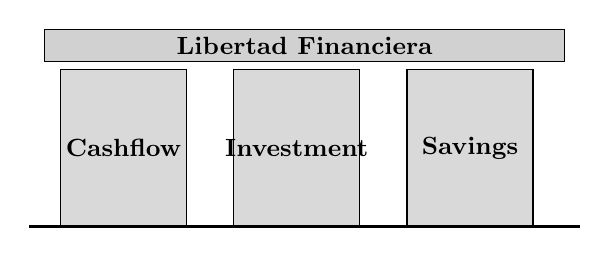
\begin{tikzpicture}[font=\small]
  \fill[accent!18] (-0.2,2.1) rectangle (6.4,2.5);
  \draw[accent] (-0.2,2.1) rectangle (6.4,2.5);
  \node[accent] at (3.1,2.3) {\bfseries Libertad Financiera};
  \foreach \x/\lbl in {0/Cashflow, 2.2/Investment, 4.4/Savings} {
    \fill[accent!15] (\x,0) rectangle (\x+1.6,2.0);
    \draw[accent] (\x,0) rectangle (\x+1.6,2.0);
    \node[accent,align=center] at (\x+0.8,1.0) {\bfseries \lbl};
  }
  \draw[accent,line width=1pt] (-0.4,0) -- (6.6,0);
\end{tikzpicture}
\caption{Los tres pilares que sostienen la libertad financiera.}
\label{fig:pillars}
\end{figure}

\textbf{Ejemplo de asignaci\'on.} Sup\'on unos ingresos de 2{,}500\,€ al mes con 1{,}500\,€ en gastos esenciales, lo que deja un Fondo de Libertad de 1{,}000\,€. Ese Fondo de Libertad puede dividirse en proporci\'on 30/40/30 como se muestra en la Tabla~\ref{tab:alloc}. Es fundamental subrayar que las cifras 30/40/30 son solo un ejemplo ilustrativo, no una f\'ormula. Cada persona tiene ingresos, compromisos, objetivos y tolerancia al riesgo distintos; una proporci\'on adecuada para una persona puede no serlo para otra. Los lectores deben dise\~nar su propia proporci\'on a partir de su situaci\'on real. Lo que no puede omitirse es que el Fondo de Libertad debe fluir siempre hacia los pilares de \textbf{Inversi\'on} y \textbf{Ahorro}; ambos son obligatorios y todo plan debe incluirlos. El tama\~no de las proporciones y la forma en que se asigna el resto (como el gasto discrecional u otros objetivos) son decisiones que cada lector puede dise\~nar libremente seg\'un su propia vida.

\begin{table}[t]
\centering
\small
\begin{tabular}{lrr}
\toprule
\rowcolor{accent!15}
\textbf{Destino} & \textbf{Proporci\'on} & \textbf{Monto (EUR)} \\
\midrule
Inversi\'on    & 30\% & 300\,€ \\
Ahorro         & 40\% & 400\,€ \\
Gasto discrecional & 30\% & 300\,€ \\
\midrule
\textbf{Fondo de Libertad total} & \textbf{100\%} & \textbf{1{,}000\,€} \\
\bottomrule
\end{tabular}
\caption{Asignaci\'on de ejemplo de un Fondo de Libertad de 1{,}000 EUR (ilustrativa).}
\label{tab:alloc}
\end{table}

\textbf{La disciplina es el coraz\'on del sistema.} Sea cual sea la asignaci\'on elegida, el factor determinante del \'exito no son las proporciones ni ninguna estrategia compleja, sino \textbf{seguir el propio sistema de forma constante durante cinco a diez a\~nos o m\'as}. El poder del DCA y del ahorro continuo solo se hace evidente cuando se deja que el tiempo y el inter\'es compuesto (compounding) hagan su trabajo. El beneficio m\'as profundo de contar con un sistema es que amortigua la influencia de las emociones, tanto la codicia en mercados alcistas como el miedo en mercados vol\'atiles, los verdaderos enemigos de las finanzas a largo plazo. Al seguir el sistema, las decisiones se basan en principios, no en sensaciones del momento. Quienes empiezan pronto y mantienen la constancia siempre superar\'an a quienes son m\'as h\'abiles pero arrancan y se detienen.

\section{Conclusi\'on}
Construir unas finanzas personales s\'olidas no requiere conocimientos financieros avanzados ni estrategias secretas, solo un sistema f\'acil de entender y una disciplina realmente practicable. Los tres pilares --- la gesti\'on del flujo de caja para conocer el Fondo de Libertad, la inversi\'on para poner el dinero a trabajar y el ahorro para reducir el riesgo --- al aplicarse juntos de manera constante, elevan gradualmente la calidad de la vida financiera a lo largo del camino.

El principio que conviene llevar siempre consigo es: \textbf{``Comienza con un sistema simple y ap\'licalo con constancia.''} El tiempo y la consistencia son los aliados m\'as poderosos de todo inversor.

\vspace{1em}
\noindent\rule{\linewidth}{0.4pt}\\
{\small\raggedright Este documento es obra de \textbf{Nonthawit Doungsodsri} --- publicado para el bien p\'ublico. M\'as informaci\'on en nonthawit.com\par}

\end{document}
